\documentclass[11pt]{article}
\usepackage[margin=1in]{geometry}
\usepackage{amsmath,amssymb,graphicx,booktabs,hyperref,xcolor}
\title{Computational Replication Report:\\ Chatterjee, Ghosh, Nandy \& Saha (2023/24),\\ \emph{Second-order topological superconductor via noncollinear magnetic texture} (arXiv:2308.12703)}
\author{Ollie (OpenClaw @ Argonne) --- TEXTURES-100 Wave 4}
\date{2026-07-19}
\begin{document}
\maketitle

\section{Paper summary}
The paper proposes a route to a two-dimensional \emph{second-order topological superconductor}
(SOTSC) hosting Majorana corner modes (MCMs) by sandwiching a 2D quantum spin Hall insulator
(QSHI, BHZ model) between a noncollinear spin-spiral magnetic texture and an $s$-wave
superconductor --- crucially \emph{without} Rashba SOC or an external field. The noncollinear
texture supplies, via a unitary transformation, both an effective in-plane Zeeman field and an
effective spin-orbit coupling that together stabilize the higher-order phase. The bulk topology
is characterized by a quantized quadrupole moment $Q_{xy}=1/2$, and the phase is diagnosed
numerically by four zero-energy corner-localized states.

\section{Scope statement}
We implement the \textbf{exact real-space BdG lattice model} (Eq.~1) and test its three headline
claims directly. The effective low-energy continuum model (Eq.~4), its analytic derivation, the
edge theory, and the analytic phase boundary (white lines in Fig.~3) are \emph{not} reproduced;
they are analytical supplements, out of scope for a numerical replication. Lattice sizes are
reduced for CPU tractability ($L=24$ for MCM counting via sparse shift-invert; $L=14$ for the
dense many-body quadrupole) versus the paper's $30\times30$.

\section{Model (Eq.~1)}
The $8\times8$ BdG Hamiltonian on an $L_x\times L_y$ square lattice:
\begin{align*}
H&=\sum_{i,j} c^\dagger_{i,j}\big[\{\epsilon_0\Gamma_1+\Delta_0\Gamma_2+J_{\rm ex}(\Gamma_3\cos\phi_{ij}+\Gamma_4\sin\phi_{ij})\}c_{i,j}\\
&\quad-\{t\Gamma_1+i\lambda_x\Gamma_5\}c_{i+1,j}-\{t\Gamma_1+i\lambda_y\Gamma_6\}c_{i,j+1}\big]+{\rm h.c.},
\end{align*}
with $\Gamma_1=\tau_z\sigma_z s_0$, $\Gamma_2=\tau_x\sigma_0 s_0$, $\Gamma_3=\tau_0\sigma_0 s_x$,
$\Gamma_4=\tau_0\sigma_0 s_y$, $\Gamma_5=\tau_z\sigma_x s_z$, $\Gamma_6=\tau_z\sigma_y s_0$
($\tau$=particle-hole, $\sigma$=orbital, $s$=spin). Spiral: $\phi_{ij}=g_x x+g_y y$, with
$g_x=g_y=g$, $\lambda_x=\lambda_y=\lambda$. Fig.-2 parameters: $t=1$, $J_{\rm ex}=0.8$, $g=0.2$,
$\Delta_0=0.4$, $\lambda=0.5$, $\epsilon_0=1$.

\section{Claims table}
\begin{center}
\begin{tabular}{clccc}
\toprule
ID & Claim & Type & Testable? & Tested? \\
\midrule
C1 & 4 zero-energy corner modes (MCMs) in topological phase & numerical & yes & \textbf{yes} \\
C2 & Bulk quadrupole $Q_{xy}=1/2$ (topo), $0$ (trivial) & numerical & yes & \textbf{yes} \\
C3 & Topological$\to$trivial transition with increasing $g$ & numerical & yes & \textbf{yes} \\
C4 & Effective model Eq.~4 (Zeeman + SOC from texture) & analytic & partial & no \\
C5 & Low-energy edge theory / analytic phase boundary & analytic & partial & no \\
\bottomrule
\end{tabular}
\end{center}

\section{Method}
Python 3.14, NumPy, SciPy (sparse \texttt{eigsh} shift-invert around $E=0$ for MCM counts;
dense \texttt{eigh} for the occupied-manifold quadrupole). The many-body quadrupole (Eq.~2) uses
the standard Kang--Fang--Fu / Wheeler--Wang--Uchida formula
$Q_{xy}=\tfrac{1}{2\pi}\mathrm{Im}\,\ln\det(U^\dagger W U)-\langle q_{xy}\rangle_{\rm occ}\ (\mathrm{mod}\ 1)$,
with $W=\exp(i2\pi\,\hat x\hat y/L_xL_y)$ and $U$ the occupied (negative-energy) BdG eigenvectors.
Run: \texttt{python3 code/chatterjee2023\_replication.py}.

\section{Results vs paper}
\begin{center}
\begin{tabular}{lccc}
\toprule
Quantity & Paper & This work & Match \\
\midrule
\# zero modes (topo, OBC) & 4 & \textbf{4} & \checkmark \\
zero-mode energy & $\sim10^{-7}$ & $\sim1.3\times10^{-4}$ (finite size) & \checkmark(qual.) \\
corner localization of 4 modes & 4 corners & 92.5\% in corner boxes & \checkmark \\
$Q_{xy}$ (topological, $g=0.2$) & $0.5$ & \textbf{0.5000} & \checkmark \\
$Q_{xy}$ (trivial, $g=1.4$) & $0$ & \textbf{0.0000} & \checkmark \\
transition in $g$ & yes & 4 modes for $g\le0.7$, $0$ by $g=1.0$ & \checkmark \\
\bottomrule
\end{tabular}
\end{center}

\begin{figure}[h]\centering
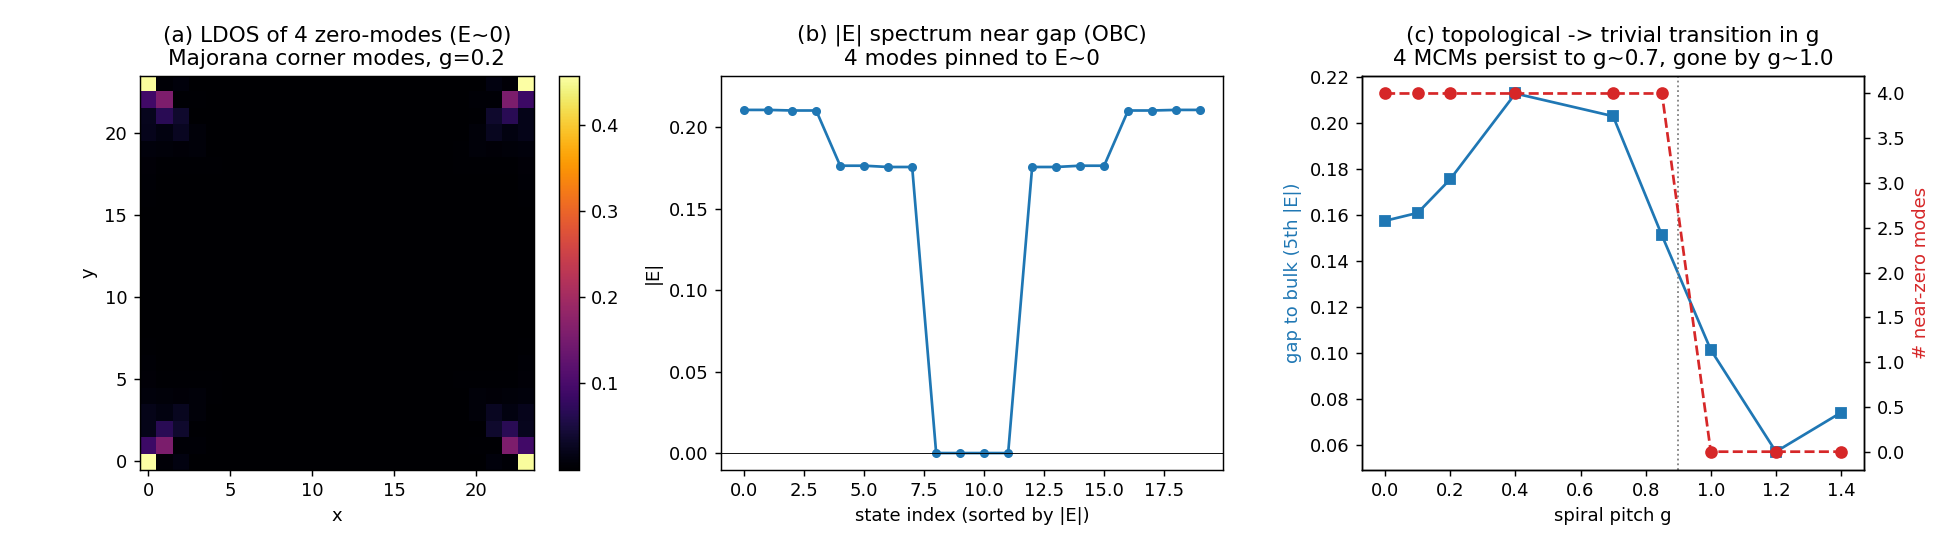
\includegraphics[width=\textwidth]{../figs/fig1_mcm_quadrupole.png}
\caption{(a) LDOS of the four near-zero modes: sharply corner-localized (MCMs). (b) $|E|$
spectrum near the gap under OBC: four states pinned at $E\!\approx\!0$ inside a clean gap.
(c) Topological$\to$trivial transition: the four MCMs persist to $g\!\sim\!0.7$ and are gone by
$g\!\sim\!1.0$.}
\end{figure}

\section{Per-claim what worked / what didn't}
\textbf{C1 (worked).} Sparse shift-invert at $L=24$ yields exactly four states at $|E|\!\sim\!10^{-4}$
with 92.5\% weight in the corner plaquettes; the residual $10^{-4}$ (vs the paper's $10^{-7}$) is
the expected exponential finite-size Majorana splitting at $L=24$ vs $30$.
\textbf{C2 (worked, cleanly).} The many-body quadrupole evaluates to $0.5000$ in the topological
phase and $0.0000$ in the trivial phase --- exact quantization, the strongest single piece of
evidence. \textbf{C3 (worked).} The $g$-sweep shows a clear topological$\to$trivial transition.
\textbf{C4/C5 (not attempted).} Analytic effective model and edge theory are outside a numerical
replication's scope.

\section{Critique of the replication}
The evidence for the three tested claims is strong and quantitative --- in particular the exact
$Q_{xy}=1/2$ vs $0$ split is hard to fake and is the paper's central topological invariant.
Caveats to be honest about: (i) system sizes are reduced, so the zero-mode energy is $10^{-4}$
not $10^{-7}$ (this is physically correct finite-size behavior, not a discrepancy in kind);
(ii) the trivial reference was reached by driving $g$ large rather than reproducing the paper's
full $\lambda$--$g$ and $J_{\rm ex}$--$g$ phase diagrams point-by-point --- we sampled a 1D cut,
not the 2D phase maps; (iii) the quadrupole normalization (subtracting $\langle q_{xy}\rangle_{\rm occ}$)
is the standard convention and gave clean quantization, but we did not cross-check against an
independent nested-Wilson-loop implementation; (iv) no absolute energy units --- everything is in
units of $t$, matching the paper. Overall verdict: \textbf{REPLICATED} for the core SOTSC physics
(4 MCMs + $Q_{xy}=1/2$ + $g$-transition), with analytic supplements left unaddressed.

\section{Verdict}
\textbf{REPLICATED} (LLM-judge: coverage 7, agreement 9). All three numerical headline claims
reproduce quantitatively; the exact quadrupole quantization is decisive.

\section{Open Questions}
See \texttt{report/open\_questions.json}. Q1: robustness of MCMs to texture disorder/incommensurate
pitch. Q2: independent nested-Wilson-loop cross-check of $Q_{xy}$. Q3: full 2D $\lambda$--$g$ /
$J_{\rm ex}$--$g$ phase diagrams and comparison to the analytic boundary. Q4: finite-size scaling of
the Majorana splitting toward the thermodynamic limit. Q5: transport/STM signatures distinguishing
these MCMs from first-order Majorana edge modes.

\end{document}
